\chapter{Desarrollo de Energym}
\label{ch:3}

En este capítulo abordaremos el proceso de desarrollo de Energym, así como las principales aportaciones realizadas en su implementación y mejora.

\section{Introducción a Energym}

Tal y como se ha adelantado en los anteriores capítulos, el principal objetivo de este proyecto consistió en el desarrollo de un entorno de ejecución de simulaciones energéticas adaptado para su uso con algoritmos de aprendizaje por refuerzo. 

Nace así \textbf{Energym}, basado en la interfaz de OpenAI Gym\footnote{OpenAI Gym es una interfaz de programación destinada al desarrollo de entornos empleados en aprendizaje por refuerzo: \url{https://gym.openai.com/}.} y destinado a servir como un marco de pruebas estándar sobre el que ejecutar algoritmos de RL/DRL en diferentes edificios y climas, favoreciendo así su evaluación y comparación. El proyecto tiene su origen en el entorno \href{https://github.com/zhangzhizza/Gym-Eplus}{Gym-Eplus} de Zhang \& Lam \cite{zhang2019whole, zhang2018practical}, cuyo \textit{back-end} fue tomado como referencia para ofrecer una nueva versión actualizada, escalable y fácilmente reutilizable.

Veamos las principales aportaciones de Energym:

\begin{itemize}
    \item \textbf{Entornos de \textit{benchmarking}}. Al igual que los entornos \href{https://gym.openai.com/envs/\#atari}{Atari} o \href{https://gym.openai.com/envs/\#mujoco}{MuJoCo} ampliamente utilizados por la comunidad de RL, Energym incorpora un conjunto de entornos para la evaluación, comparativa y prueba de algoritmos de RL/DRL en control energético de edificios. Estos entornos incluyen diferentes edificios, climas y espacios de acciones.
    \item \textbf{Flexibilidad en la experimentación}. Energym permite la personalización de diferentes aspectos de la simulación, tales como la función de recompensa empleada o la selección de las variables que conforman las observaciones de los agentes.
    \item \textbf{Compatibilidad con diferentes motores de simulación}. Aunque actualmente sólo se ha implementado la conexión con \href{https://energyplus.net/}{EnergyPlus}, el objetivo es que Energym pueda ser empleado con diferentes motores de simulación, como \href{https://www.openmodelica.org/}{OpenModelica} o \href{https://es.mathworks.com/products/simulink.html}{Simulink}.
    \item \textbf{Integración con \href{https://stable-baselines3.readthedocs.io}{Stable Baselines3}}. Energym cuenta con diferentes funcionalidades adaptadas a esta librería de RL (ej. \textit{callbacks}) con el fin de poder probar fácilmente los entornos implementados.
\end{itemize}

Una vez definidas las principales características de Energym, pasemos a estudiar su funcionamiento. Como se muestra en la Figura \ref{fig:energym-ecosystem}, el ecosistema de simulación planteado consta de los siguientes elementos:

\begin{figure}
    \centering
    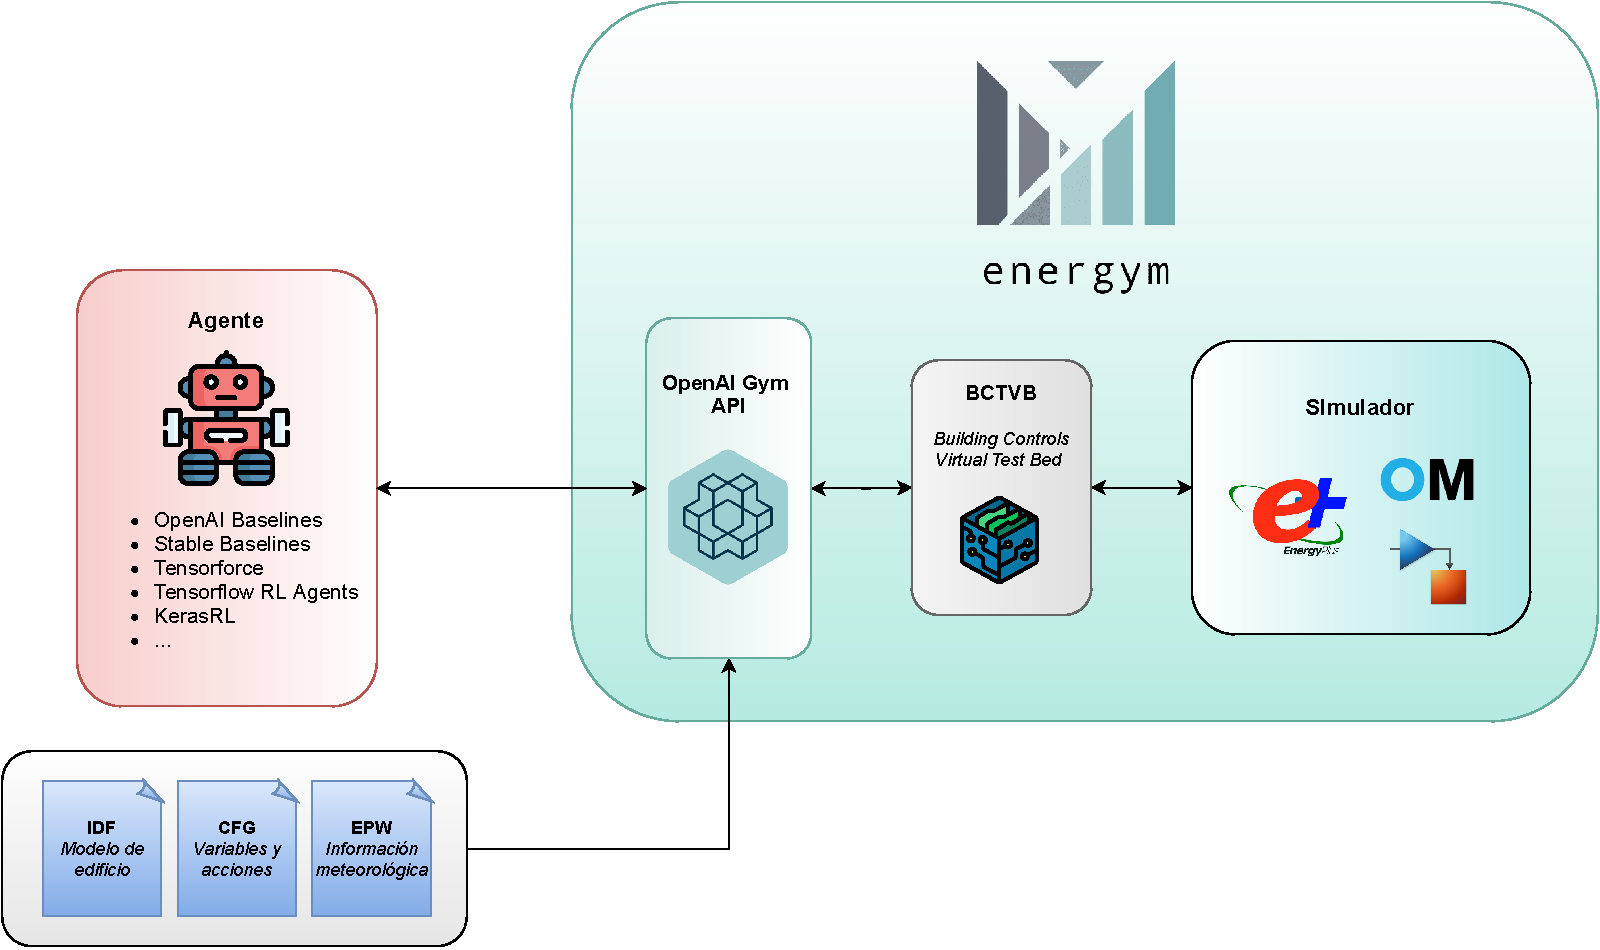
\includegraphics[width=\textwidth]{imagenes/energym-diagram.pdf}
    \caption{Elementos que componen el ecosistema de Energym}
    \label{fig:energym-ecosystem}
\end{figure}

\begin{itemize}
    \item Un \textbf{agente} que interactúa con el entorno. Su implementación puede llevarse a cabo mediante diferentes librerías de DRL, tales como \href{https://github.com/openai/baselines}{OpenAI Baselines}, \href{https://github.com/DLR-RM/stable-baselines3}{Stable Baselines}, \href{https://www.tensorflow.org/agents}{Tensorflow Agents},  \href{https://github.com/keras-rl/keras-rl}{KerasRL}, etc.
    \item Una serie de \textbf{ficheros de configuración} que serán empleados en la simulación:
        \begin{itemize}
            \item Un fichero \texttt{.idf} (\textit{Input Data File}, IDF) con el modelo del edificio empleado en la simulación.
            \item Un fichero \texttt{.cfg} con información sobre las acciones, variables de entrada y salida a emplear, sus rangos, etc.
            \item Un fichero \texttt{.epw} (\href{https://energyplus.net/weather}{\textit{EnergyPlus Weather}}, EPW) con información meteorológica empleada en la simulación.
        \end{itemize}
    Todo entorno queda definido por el edificio, variables de entrada y salida, tipos de acciones (discretas o continuas) y clima especificados en estos ficheros.
    \item El entorno de simulación \textbf{Energym}, desarrollado bajo la interfaz de OpenAI Gym y conectado a un simulador (EnergyPlus, OpenModelica, Simulink...) por medio de BCTVB (\textit{Building Controls Virtual Test Bed}). BCVTB es un \textit{middleware} \textit{open source} que permite el acoplamiento de diferentes sistemas de simulación distribuidos. En nuestro caso, su uso reside en la conexión entre el entorno de simulación y el simulador empleado\footnote{Para más información, consúltese: \url{https://simulationresearch.lbl.gov/bcvtb}.}.
\end{itemize}

Así, la interacción entre estos elementos se realiza tal y como se muestra en la Figura \ref{fig:operation-diag}: el agente interactúa con Energym modificando una serie de variables de entrada y recibe observaciones con el valor de las variables de salida proporcionadas tras la simulación. Por otro lado, en base a las dinámicas del entorno se genera una recompensa que el agente tratará de maximizar.

\begin{figure}
    \centering
    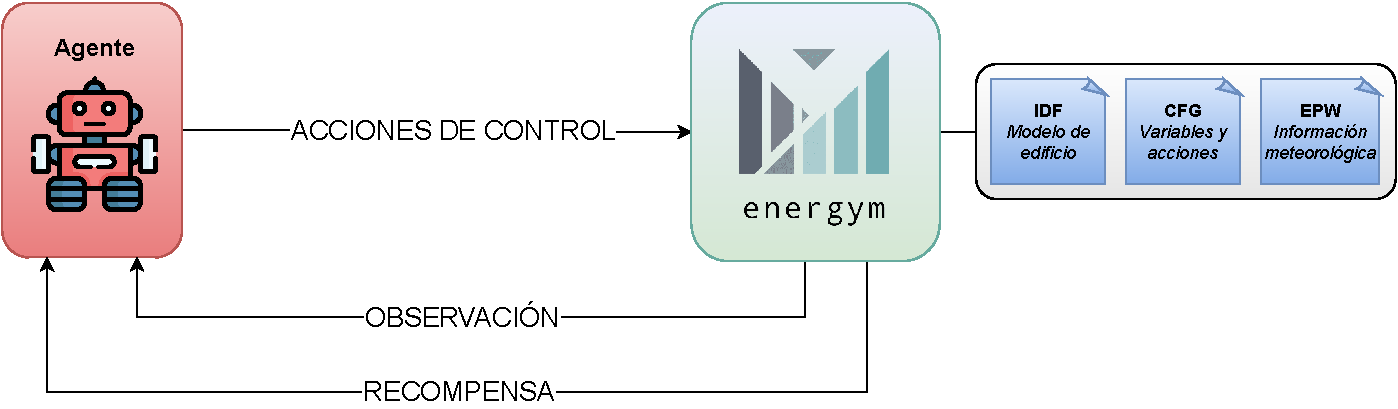
\includegraphics[width=\textwidth]{imagenes/operation-diagram.pdf}
    \caption{Proceso de simulación}
    \label{fig:operation-diag}
\end{figure}

Cabe destacar que, hasta el momento, no existe ninguna propuesta similar a Energym, lo que supone una importante contribución en este campo. Además, el hecho de distribuirse como código abierto abre la oportunidad a futuras aportaciones por parte de usuarios interesados en colaborar en su desarrollo. El principal objetivo de Energym es ofrecer un entorno de simulación sencillo, eficiente y flexible, de tal forma que cualquier usuario que desee utilizarlo en sus propios proyectos pueda descargar el código y modificar la configuración para adecuar Energym a sus objetivos.

Finalmente, Energym abre la puerta a un gran número de posibles experimentaciones: comparativa de algoritmos de RL/DRL sobre unas mismas condiciones; estudio de la influencia del clima en el control energético; análisis de las variables que más influyen en el aprendizaje; comparativa de desempeño para espacios de acciones discretos y continuos, y un largo etcétera.

\section{Organización y metodología de trabajo}

La implementación de Energym llevada a cabo en el marco de este proyecto supuso la colaboración como parte de su equipo de desarrollo. Así, partiendo de un proyecto iniciado el 23 de enero de 2021 y una serie de ideas generales sobre los objetivos a perseguir, se pasó a formar parte de su desarrollo.

El equipo de trabajo del cual se pasó a formar parte durante esta parte del trabajo estuvo compuesto por los siguientes integrantes:

\begin{itemize}
    \item Javier Jiménez: creador del proyecto, encargado de gestionar el repositorio de Energym, así como de dirigir su desarrollo en líneas generales.
    \item Alejandro Campoy: incorporado al desarrollo de Energym a partir del 12 de abril.
    \item Juan Gómez y Miguel Molina: supervisores del proyecto.
\end{itemize}

La colaboración con el equipo de desarrollo se llevó siguiendo una comunicación continua por medio de herramientas colaborativas como Slack o GitHub. No se trató de un desarrollo al uso, sino que se siguió una forma de trabajo propia de entornos profesionales, siguiendo una metodología de desarrollo basada en \textit{issues}/\textit{pull requests}, integración continua, versionado y desarrollo en ramas independientes, etc. En las Figuras \ref{fig:git1}, \ref{fig:git2} y  \ref{fig:git3} se muestra una perspectiva general del repositorio.

\begin{figure}
    \centering
    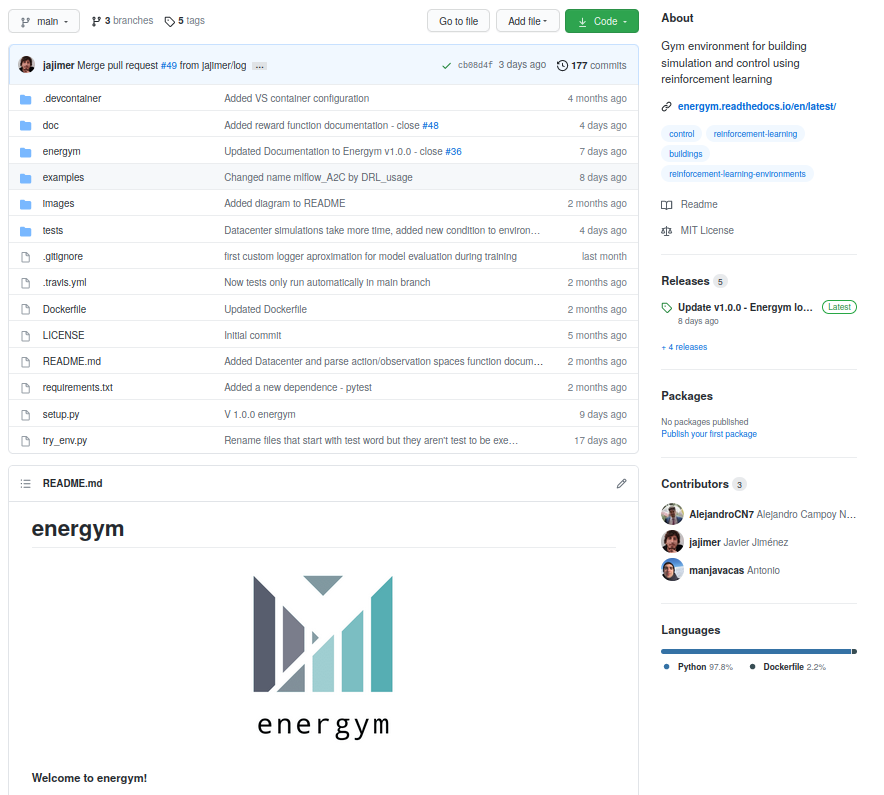
\includegraphics[width=\textwidth]{imagenes/git.png}
    \caption{Repositorio de Energym en GitHub}
    \label{fig:git1}
\end{figure}

\begin{figure}
    \centering
    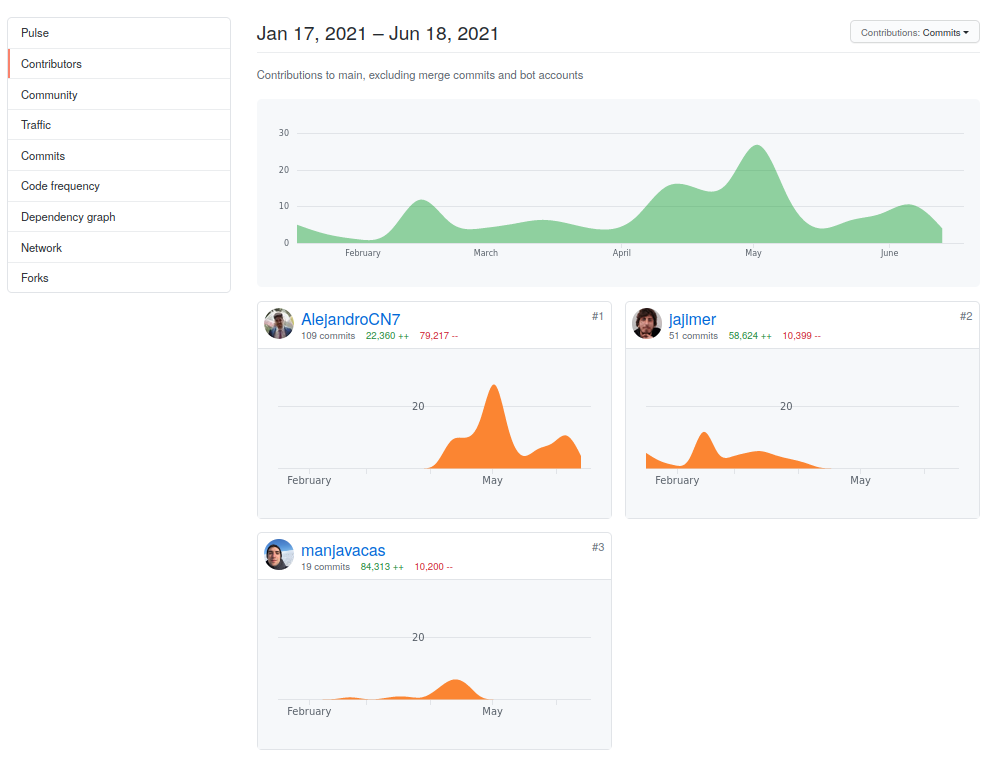
\includegraphics[width=\textwidth]{imagenes/git-contributions.png}
    \caption{Contribuciones al repositorio}
    \label{fig:git2}
\end{figure}

\begin{figure}
    \centering
    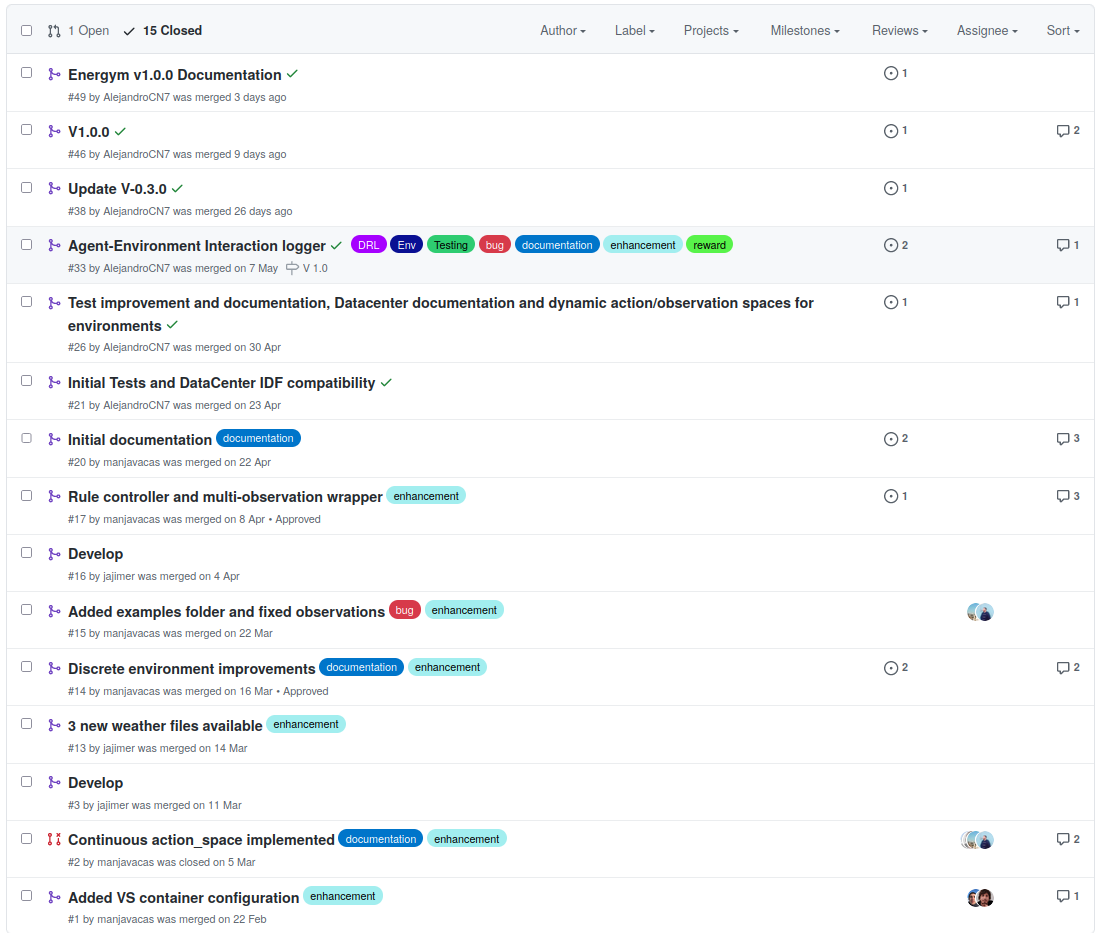
\includegraphics[width=\textwidth]{imagenes/git-pull-requests.png}
    \caption{Desarrollo basado en \textit{pull requests}}
    \label{fig:git3}
\end{figure}

En la Figura \ref{fig:git2} puede observarse cómo la primera parte del desarrollo fue principalmente llevada a cabo por Javier Jiménez, creador del proyecto; posteriormente, el autor de este trabajo tomó el relevo en su implementación (puede verse una mayor frecuencia de contribuciones entre febrero y mayo) para, posteriormente, dar el relevo a Alejandro Campoy como principal desarrollador desde el mes de abril.

\section{Contribuciones al desarrollo}

Como parte de las aportaciones realizadas en el desarrollo de Energym, destacan las siguientes tareas:

\subsection{Imagen Docker}

Un primer paso fue la implementación de la imagen Docker empleada para desarrollar y utilizar Energym, facilitando la gestión de dependencias y el desarrollo dentro de un entorno aislado. 
    
Docker permite el despliegue de aplicaciones en contenedores, ofreciendo modularidad, una rápida implementación y un desarrollo flexible. Simplemente es necesario definir un fichero Dockerfile donde se especifiquen las operaciones a realizar una vez inicializado el contenedor (instalación de dependencias, declaración de variables de entorno, etc.) para, posteriormente, poder interactuar con el entorno virtualizado que Docker ofrece.
    
Así, se propuso la implementación de una imagen Docker que permitiese utilizar Energym en un entorno cerrado, gestionándose de forma automática aspectos tales como la instalación de EnergyPlus y BCVTB, o la declaración de las variables de entorno empleadas por Energym. 
    
Finalmente, se incluyó en el repositorio la configuración necesaria para automatizar la construcción y despliegue del contenedor en Visual Studio Code de forma rápida y sencilla.

\subsection{Desarrollo de entornos de simulación}
\label{sec:entornos}
    
Posteriormente, se procedió al desarrollo de los entornos basados en espacios de acciones continuos y discretos. Como ya mencionamos en la sección \ref{sec:formulacion}, el problema de regulación de \textit{setpoints} en control HVAC puede formularse considerando un espacio de acciones discreto o continuo. El objetivo perseguido en el desarrollo de Energym fue el de implementar ambos, de cara a evaluar el desempeño de algoritmos de DRL que únicamente operan en un tipo de espacio de acciones (por ejemplo, DQN en entornos discretos, o DDPG en continuos). Otro objetivo considerado fue el de evaluar los resultados obtenidos por un mismo algoritmo en cada tipo de entorno (por ejemplo, A2C).
    
Para los entornos basados en acciones discretas, los rangos de temperatura se fijaron de acuerdo a los propuestos en \cite{center2013determining}. En este caso, un total de 10 configuraciones componen el espacio de acciones\footnote{Los espacios de acciones pueden configurarse a voluntad modificando el fichero \texttt{.cfg} empleado por Energym.}, donde cada una está compuesta por una tupla $<setpoint_{calor},\ setpoint_{frio}>$ (ver Tabla \ref{tb:disc-actions}).
    
    \begin{table}
        \centering
        \caption{Espacio de acciones discreto empleado por defecto}
        \label{tb:disc-actions}
        \begin{tabular}{ccc}
        N & \textit{Setpoint calor} & \textit{Setpoint frío} \\ \hline
        0 & 15 & 30 \\ \hline
        1 & 16 & 29 \\ \hline
        2 & 17 & 28 \\ \hline
        3 & 18 & 27 \\ \hline
        4 & 19 & 26 \\ \hline
        5 & 20 & 25 \\ \hline
        6 & 21 & 24 \\ \hline
        7 & 22 & 23 \\ \hline
        8 & 22 & 22 \\ \hline
        9 & 21 & 21 \\ \hline
        \end{tabular}
    \end{table}
    
Con respecto a los entornos continuos, el ajuste de los \textit{setpoints} quedó acotado a los intervalos que se muestran en la Tabla \ref{tb:cont-actions}. Dentro de dichos intervalos, cada \textit{setpoint} podrá tomar un valor continuo determinando, lo que incrementa más que considerablemente el número de combinaciones acción--estado que podrán darse dentro del entorno.
    
\begin{table}
    \centering
    \caption{Espacio de acciones continuo empleado por defecto}
    \label{tb:cont-actions}
    \begin{tabular}{llll}
    N & \textit{Setpoint} & Mín. & Max. \\ \hline
    0 & Calor & 15,0 & 22,5 \\ \hline
    1 & Frío & 22,5 & 30,0 \\ \hline
    \end{tabular}
\end{table}

Una vez visto el tipo de acciones que podemos ejecutar sobre el entorno, otros elementos configurables empleados por Energym son: las \textbf{variables} que definen una observación, el \textbf{edificio} empleado para la simulación, y el \textbf{clima}, los cuales abordaremos en detalle en el Capítulo \ref{ch:4}. Además, es posible (y recomendable de cara a favorecer la generalización en el aprendizaje) simular entornos estocásticos donde los datos meteorológicos presentes en el fichero \texttt{.epw} son ligeramente modificados en cada episodio a partir de \textbf{ruido} gaussiano (con media $0$ y desviación estándar $2,5$).

Finalmente, los entornos de simulación considerados en este proyecto son los mostrados en la Tabla \ref{tb:entornos}, de acuerdo a las posibles combinaciones de espacio de acciones y clima\footnote{Tipos de clima acordes a la clasificación del \href{https://www.energycodes.gov/development/commercial/prototype_models}{DOE}.}. Profundizaremos en estos ellos en el Capítulo \ref{ch:4}.
   
%%%

\begin{landscape}
    \begin{table}
    \centering
    \caption{Entornos empleados en este proyecto}
    \label{tb:entornos}
    \begin{tabular}{llllll}
    \multicolumn{1}{c}{\textbf{Entorno}} & \multicolumn{1}{c}{\textbf{Localización}} & \multicolumn{1}{c}{\textbf{IDF}} & \multicolumn{1}{c}{\textbf{Clima}} & \multicolumn{1}{c}{\textbf{Acciones}} & \multicolumn{1}{c}{\textbf{Período}} \\ \hline
    Eplus-discrete-stochastic-hot-v1 & Arizona, USA & 5ZoneAutoDXVAV.idf & Hot dry (2B) + ruido & Discrete(10) & 01/01 - 31/12 \\
    Eplus-discrete-stochastic-mixed-v1 & New York, USA & 5ZoneAutoDXVAV.idf & Mixed humid (4A) + ruido & Discrete(10) & 01/01 - 31/12 \\
    Eplus-discrete-stochastic-cool-v1 & Washington, USA & 5ZoneAutoDXVAV.idf & Cool marine (5C) + ruido & Discrete(10) & 01/01 - 31/12 \\ \hline
    Eplus-continuous-stochastic-hot-v1 & Arizona, USA & 5ZoneAutoDXVAV.idf & Hot dry (2B) + ruido & Box(2) & 01/01 - 31/12 \\
    Eplus-continuous-stochastic-mixed-v1 & New York, USA & 5ZoneAutoDXVAV.idf & Mixed humid (4A) + ruido & Box(2) & 01/01 - 31/12 \\
    Eplus-continuous-stochastic-cool-v1 & Washington, USA & 5ZoneAutoDXVAV.idf & Cool marine (5C) + ruido & Box(2) & 01/01 - 31/12 \\ \hline
    \end{tabular}%
    \end{table}
\end{landscape}

%%%

\subsection{Gestión de los ficheros de configuración}

Esta tarea supuso la lectura y adaptación de los ficheros de configuración (\texttt{.idf}, \texttt{.cfg} y \texttt{.epw}) utilizados por Energym. Por un lado, requirió la búsqueda y uso de librerías destinadas a una lectura eficiente de los ficheros IDF empleados por Energym (por ejemplo, \href{https://pypi.org/project/opyplus/}{\textit{opyplus}}). También se realizaron modificaciones en el modelo de edificio para adaptarlo a la experimentación que posteriormente sería llevada a cabo, como la ampliación del período de simulación a 1 año.

Por otro lado, a las variables devueltas por EnergyPlus como observación en cada \textit{timestep} se añadieron valores adicionales, como la hora o fecha de cada día simulado. Esta información no sólo se incorporó como una variable más a emplear en el aprendizaje, sino también con el fin de añadir a las simulaciones una mayor trazabilidad y facilitar su estudio desde diferentes perspectivas temporales. Por ejemplo: considerar en qué meses el rendimiento obtenido es peor, si existe algún tipo de estacionalidad en la recompensa obtenida, etc.
    
\subsection{Limpieza y adaptación del \textit{back-end}}

De especial relevancia fue la limpieza y adaptación del código \textit{back-end} heredado del repositorio de \href{https://github.com/zhangzhizza/Gym-Eplus}{Gym-Eplus}. El \textit{back-end} de este proyecto fue reutilizado para establecer la conexión entre Energym y EnergyPlus a través de BCVTB, tal y como se muestra en la Figura \ref{fig:backend}.
    
\begin{figure}
    \centering
    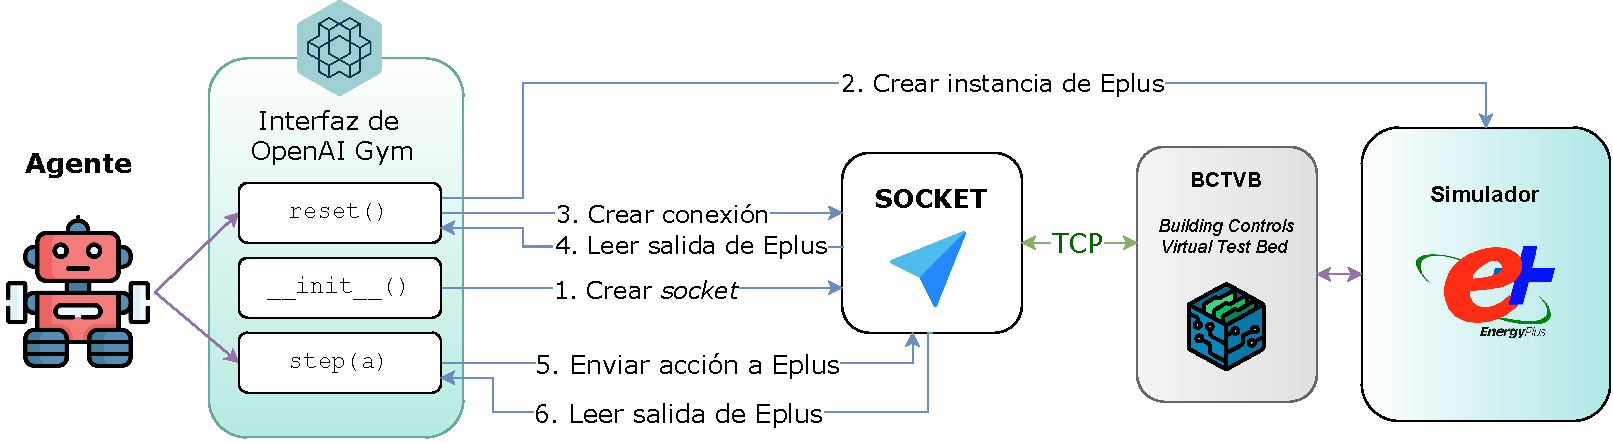
\includegraphics[width=\textwidth]{imagenes/backend.pdf}
    \caption{Interacción con el \textit{back-end} de Energym, heredado de Gym-Eplus. Imagen modificada de \cite{zhang2019whole}}
    \label{fig:backend}
\end{figure}

Al partir de código heredado, fue necesaria una completa interpretación del \textit{back-end} del proyecto original antes de abordar su adaptación y optimización. Posteriormente, se llevó a cabo su reorganización, eliminando aquellas partes de código no empleadas en nuestro proyecto y modificando otras para poder ser utilizadas con Energym. Finalmente, esta parte del proyecto pasó a ser documentada.

\subsection{Documentación}

De cara a contar con un documento de referencia que permitiese detallar el funcionamiento de Energym a la comunidad, se desarrolló la primera versión de la documentación de la librería utilizando \href{https://www.sphinx-doc.org}{\textit{Sphinx}}. Así, una vez implementado el núcleo funcional de Energym, se procedió a documentar sus principales componentes. \textit{Sphinx} ofrece numerosas facilidades para elaborar la documentación de código, siempre y cuando se parta de un código comentado en un formato estándar como \href{https://www.sphinx-doc.org/en/master/usage/extensions/example_numpy.html?highlight=numpy#example-numpy-style-python-docstrings}{Numpy} o \href{https://www.sphinx-doc.org/en/master/usage/extensions/example_google.html#example-google}{Google}.

La documentación generada fue publicada en la plataforma \href{readthedocs.org}{\textit{Read the Docs}} (ver Figura \ref{fig:readthedocs}), la cual permite su alojamiento de forma gratuita y la sincronización automática con el repositorio en el que se aloja el proyecto\footnote{La documentación de Energym se encuentra actualizada y puede consultarse en el siguiente enlace: \url{https://energym.readthedocs.io/}.}.

\begin{figure}
    \centering
    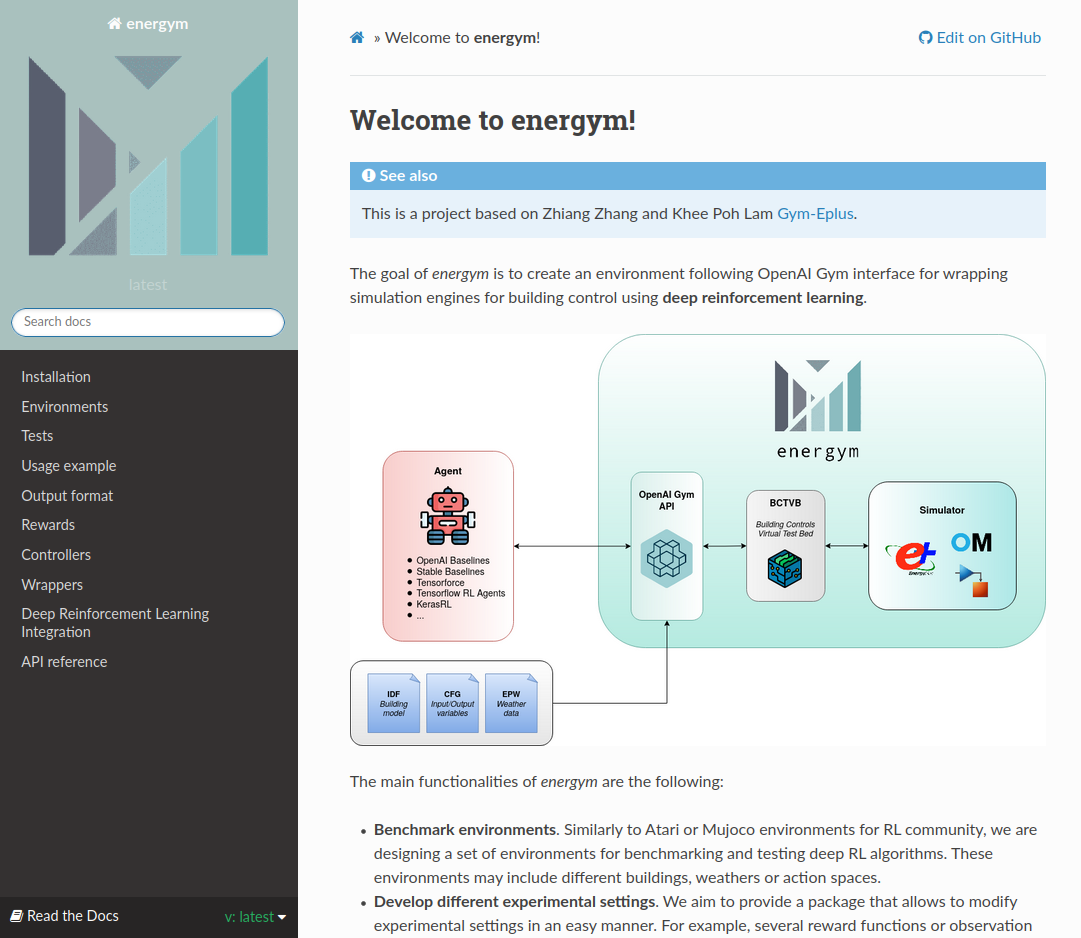
\includegraphics[width=\textwidth]{imagenes/readthedocs.png}
    \caption{Documentación de Energym alojada en \textit{Read the Docs}}
    \label{fig:readthedocs}
\end{figure}

Finalmente, a la elaboración de la documentación inicial se sumó la implementación de una serie \textit{scripts} de ejemplo destinados a ilustrar el funcionamiento de Energym en diferentes contextos. Estos serían empleados para probar la integración de Energym con MLflow y Tensorboard, ejemplificar el uso de \textit{wrappers}, o mostrar la integración de Energym con Stable Baselines3, como veremos más adelante.

\subsection{Controlador basado en reglas}
Un aspecto importante a la hora de poder evaluar la eficiencia de algoritmos de DRL en control HVAC es tener como referencia un controlador basado en reglas con respecto al cual poder comparar. Esta tarea supuso el desarrollo de dicho controlador, cuyo funcionamiento se detalla en el Algoritmo \ref{alg:reglas}. De nuevo, se tomaron como referencia los rangos de temperatura expuestos en \cite{center2013determining}.

\begin{algorithm}
\caption{Controlador basado en reglas}
\label{alg:reglas}
\DontPrintSemicolon
\LinesNumbered
\KwIn{$s$: una observación del entorno}
\KwOut{$accion$: la combinación de \textit{setpoints} a ajustar}

$t \leftarrow$ obtener temperatura exterior de $s$\;

    \If{$t < 15$}{
        $accion = (19,21)$\;
    }
    \ElseIf{$t < 20$}{
        $accion = (20,22)$\;
    }
    \ElseIf{$t < 26$}{
        $accion = (21,23)$\;
    }
    \ElseIf{$t < 30$}{
        $accion = (26,30)$\;
    }
    \Else{
        $accion = (24,26)$\;
    }

\Return{accion}

\end{algorithm}

Como puede observarse, un controlador basado en reglas ajusta los \textit{setpoints} en base a la temperatura exterior del entorno. La ventaja de este enfoque basado en reglas es su aplicabilidad en la mayoría de sistemas, la clara interpretación de las reglas, así como su flexibilidad para ajustarse a cualquier tipo de dispositivo HVAC \cite{mavrik2011advanced}. 

No obstante, este tipo de controladores suelen ser ineficientes en la práctica, debido a la complejidad de la dinámica térmica de los edificios y a las perturbaciones heterogéneas que puedan darse en el entorno. Tal y como se explica en \cite{wei2017deep, yang2015reinforcement}, el rendimiento y fiabilidad de estos enfoques dependen en gran medida de la precisión del modelo térmico del edificio, el cual no sólo debe ser preciso sino también eficiente. Además, la temperatura del edificio puede verse afectada por muchos factores no contemplados por estos sistemas, como la estructura y materiales del edificio, la humedad, la intensidad de la radiación solar o las ganancias de calor debidas a los ocupantes del edificio. Como resultado, la temperatura del edificio termina por presentar comportamientos aleatorios debido a una modelización incompleta. 

Concluimos, por tanto, enfatizando la dificultad para desarrollar un controlador basado en reglas lo suficientemente preciso y eficiente para un control eficaz de la climatización en tiempo real. De aquí parte la idea de desarrollar algoritmos de RL/DRL que traten de mejorar estas propuestas, siempre y cuando se parta de un control basado en reglas a partir del cual poder comparar los resultados obtenidos (tanto en términos de confort como de consumo).

\subsection{\textit{Wrappers}}

OpenAI Gym permite extender los entornos convencionales de forma modular por medio de \textit{wrappers}. Las clases que heredan de \texttt{gym.Wrapper} permiten al programador personalizar observaciones (\texttt{gym.ObservationWrapper)}, acciones (\texttt{gym.ActionWrapper)} y recompensas (\texttt{gym.RewardWrapper)}, sobrescribiendo sus implementaciones por defecto.

En el caso de Energym, se implementaron una serie de \textit{wrappers} de cara a extender las funcionalidades del entorno por defecto\footnote{Su implementación puede consultarse en: \url{https://github.com/jajimer/energym/blob/main/energym/utils/wrappers.py}}:

\begin{itemize}
    \item \texttt{NormalizeObservation}: \textit{wrapper} destinado a normalizar los valores de las variables que componen cada observación. El objetivo perseguido con este \textit{wrapper} es favorecer el entrenamiento de los algoritmos de DRL, reduciendo la variabilidad de los valores empleados. 
    
    Un problema inicial fue decidir qué rangos emplear para normalizar cada valor mediante min--max:
    
    \begin{equation}
        x_{norm} = \frac{x - min}{max - min}
    \end{equation}
    
    Para resolver este problema, se llevó a cabo una aproximación empírica basada la ejecución de múltiples simulaciones con un agente aleatorio. Partiendo de los registros de estas simulaciones, fue posible conocer los valores mínimo y máximo del dominio de cada variable, y emplearlos así para normalizar.
    
    Finalmente, se comprobó que este \textit{wrapper} mejoraba los resultados obtenidos por los agentes con respecto al uso de observaciones por defecto.
    
    \item \texttt{MultiObsWrapper}: este \textit{wrapper} permite agrupar múltiples observaciones y utilizar su información de forma combinada para favorecer el entrenamiento. Si bien se trata de un tipo de \textit{wrapper} especialmente útil en entornos como Atari o MuJoCo (ya que sucesivas observaciones agrupadas pueden ayudar a determinar, por ejemplo, el movimiento de un objeto), en el caso de Energym el uso de este tipo de \textit{wrapper} no supuso mejoras significativas sobre el rendimiento de los agentes.
    
    \item \texttt{LoggerWrapper}: recoge información relacionada con la simulación episodio a episodio y la almacena de forma persistente en formato \texttt{.csv}. Resultó especialmente útil para evaluar el rendimiento de los diferentes agentes.
\end{itemize}

\subsection{Integración con \textit{Stable Baselines3} y \textit{Tensorboard}}

Como se detallará en profundidad en el Capítulo \ref{ch:4}, una de las principales tareas realizadas fue la experimentación e integración de Energym con \href{https://stable-baselines3.readthedocs.io}{Stable Baselines3}. Se trata de una de las librerías más utilizadas en el ámbito del DRL, ya que contiene implementaciones basadas en PyTorch, eficientes y bien documentadas de un importante número de algoritmos de este ámbito. 

La mayor parte de los algoritmos disponibles en Stable Baselines3 fueron probados y evaluados empleando Energym en diferentes entornos. Así, a la programación de diferentes \textit{scripts} destinados al entrenamiento y evaluación de los algoritmos, se sumó el desarrollo en paralelo de un \textit{callback} de evaluación destinado a procesar toda la información posible obtenida durante el entrenamiento, tanto desde el punto de vista del entorno como de los agentes\footnote{Para más información, véase:  \url{https://energym.readthedocs.io/en/latest/pages/deep-reinforcement-learning.html}.}. 

Así, las variables monitorizadas incluyen aspectos de interés como las observaciones percibidas por el agente, las acciones llevadas a cabo en cada \textit{timestep}, los valores de entrenamiento de las redes neuronales, medidas de rendimiento, o las recompensas obtenidas.

Una de las principales ventajas de Stable Baselines3 es que cuenta con integración con \href{https://www.tensorflow.org/tensorboard}{TensorBoard}, una potente herramienta de visualización orientada, en este caso, a la monitorización del proceso de entrenamiento de los diferentes algoritmos. De esta forma, tal y como se muestra en la Figura \ref{fig:tensorboard}, se pudo llevar a cabo el seguimiento y comparación del entrenamiento de los algoritmos empleados.

\begin{figure}
    \centering
    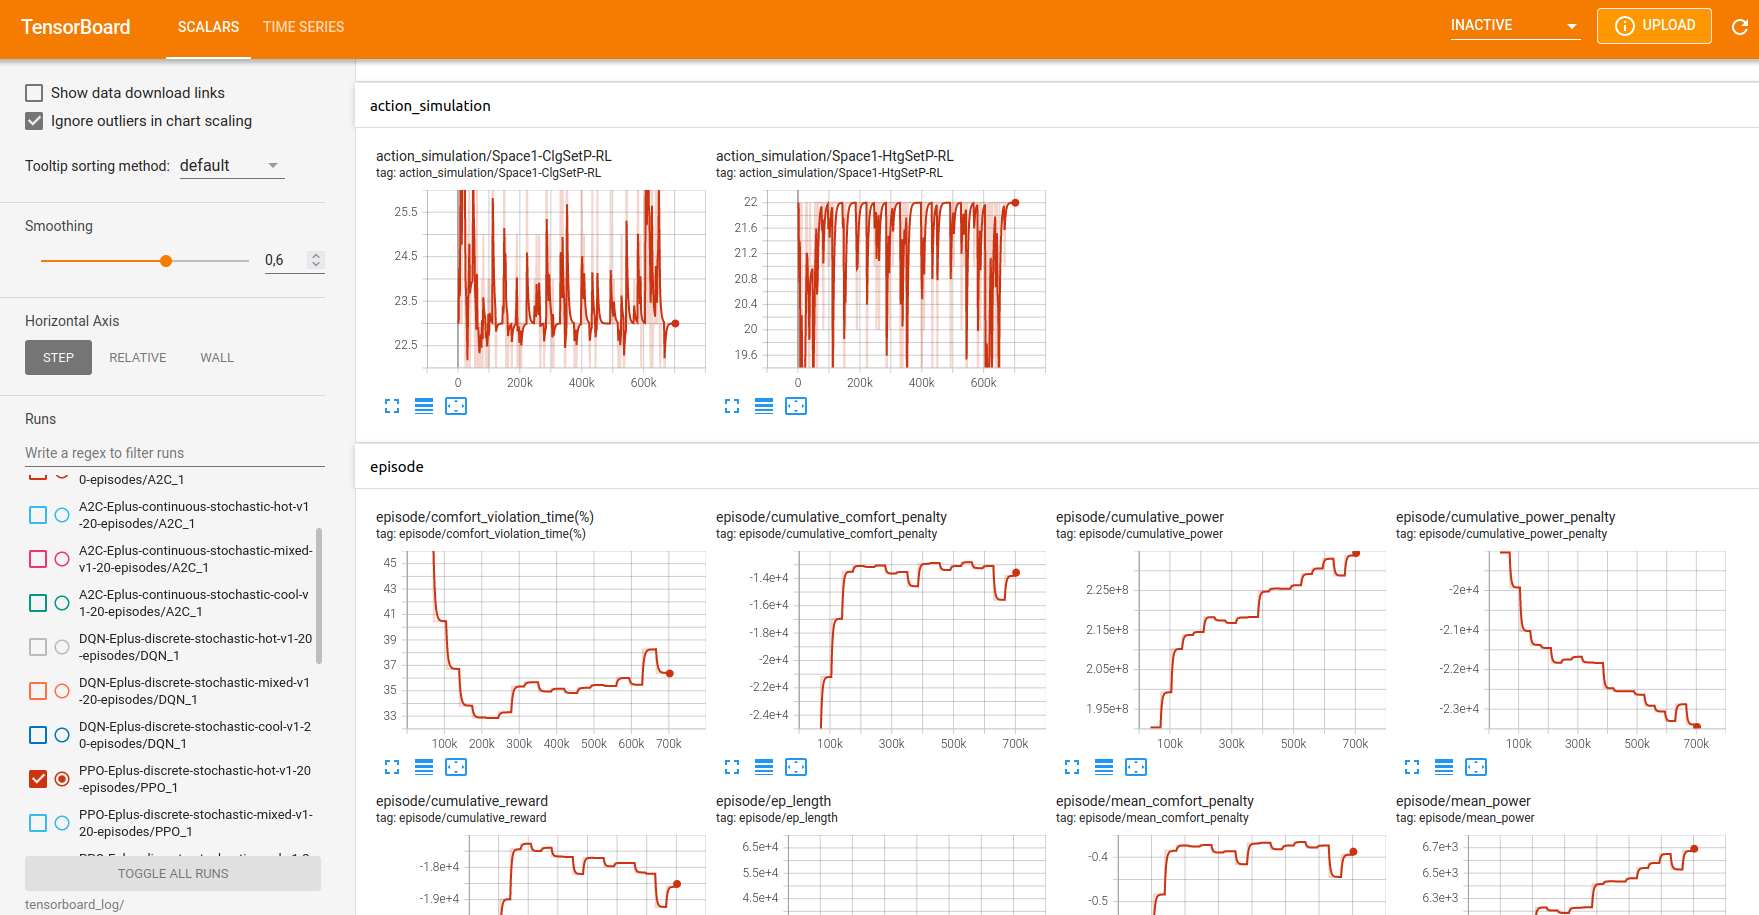
\includegraphics[width=\textwidth]{imagenes/tensorboard.png}
    \caption{Monitorización del entrenamiento mediante TensorBoard}
    \label{fig:tensorboard}
\end{figure}

Finalmente, veamos la información recogida y mostrada por TensorBoard, la cual se divide en los siguientes grupos:

\begin{itemize}
    \item Registro de las acciones empleadas por el agente durante la simulación.
    \item Medidas de rendimiento recopiladas episodio a episodio:
    \begin{itemize}
        \item Porcentaje de tiempo bajo violación de confort, donde la temperatura estuvo fuera de los límites de confort definidos.
        \item Valor medio y suma acumulada de las penalizaciones por confort durante un episodio completo.
        \item Consumo energético total a lo largo de cada episodio.
        \item Valor medio y suma acumulada de las penalizaciones por consumo energético.
        \item Recompensa media y acumulada.
        \item Duración (en \textit{timesteps}) de cada episodio.
    \end{itemize}
    \item Valor de las variables observadas durante la simulación (dependientes del entorno).
    \item Valores normalizados de las variables observadas, en caso de emplearse el \textit{wrapper} de normalización previamente mencionado.
    \item Métricas ofrecidas por Stable Baselines3 relacionadas con cada algoritmo (por ejemplo, la variación del ratio de exploración en DQN).
    \item Tiempo de ejecución.
    \item Información sobre los valores de entrenamiento de las redes neuronales, ofrecida por Stable Baselines3.
    \item Medidas de rendimiento obtenidas en los episodios de evaluación, en caso de utilizar el \textit{callback} \texttt{EvalLoggerCallback} durante el entrenamiento\footnote{Para más información sobre los \textit{callbacks} ofrecidos por Stable Baselines3, véase: \url{https://stable-baselines.readthedocs.io/en/master/guide/callbacks.html}.}. Este \textit{callback} permite evaluar periódicamente el rendimiento del agente entrenado, empleando un entorno de \textit{test} independiente. A su vez, preserva el mejor modelo obtenido hasta el momento en un directorio indicado por el usuario.
\end{itemize}
    
\subsection{Integración con MLflow}

Por último, con el fin de realizar un seguimiento de los experimentos ejecutados y registrar la configuración de los diferentes algoritmos, se decidió emplear \href{https://mlflow.org/}{MLflow}. Se trata de una plataforma \textit{open source} orientada a la gestión del ciclo de vida en proyectos de \textit{machine learning} y ampliamente utilizada en el ámbito del \href{https://ml-ops.org/}{MLOps}. Su uso es similar al de otras herramientas como \href{https://neptune.ai/}{Neptune}, \href{https://www.comet.ml}{Comet}, \href{https://polyaxon.com/}{Polyaxon}, \href{https://valohai.com/}{Valohai}, \href{https://metaflow.org/}{Metaflow} o \href{https://wandb.ai/site}{WandB}. No obstante, a pesar de las numerosas posibilidades existentes, el hecho de ser \textit{open source}, así como su simplicidad y flexibilidad ante las necesidades de este proyecto fueron las principales razones que llevaron a elegir esta herramienta.

Atendiendo a sus principales funcionalidades, MLflow permite registrar experimentos (\textit{runs}) manteniendo un listado personalizable de las configuraciones empleadas en cada ejecución. También permite comparar su desempeño, elaborar gráficos comparativos entre diversas parametrizaciones, así como almacenar, gestionar y desplegar diferentes versiones de los modelos entrenados.

En el marco de este proyecto, MLflow (y, en especial, su módulo \textit{Model Registry}) resultó de especial interés a la hora de mantener un registro estable de los experimentos realizados y sus configuraciones. Cabe destacar que MLflow no es una herramienta exclusivamente orientada a la gestión de modelos de aprendizaje por refuerzo, pero que contó con la suficiente flexibilidad como para cubrir las necesidades de este proyecto. De esta forma, su principal uso consistió en el registro y estudio de los hiperparámetros empleados en el entrenamiento de los modelos de DRL, así como de las métricas de evaluación empleadas, como la recompensa media o el tiempo de entrenamiento.

Desde un punto de vista práctico, simplemente fue necesario especificar qué parámetros y métricas debían ser empleados durante los experimentos para que MLflow se encargase de su registro y monitorización\footnote{Véase el ejemplo en código disponible en la documentación de Energym: \url{https://energym.readthedocs.io/en/latest/pages/deep-reinforcement-learning.html\#how-use}.}.

Finalmente, en la Figura \ref{fig:mlflow} se muestra el listado de ejecuciones registradas en MLflow, correspondientes a los experimentos que abordaremos en el siguiente capítulo.

\begin{figure}
    \centering
    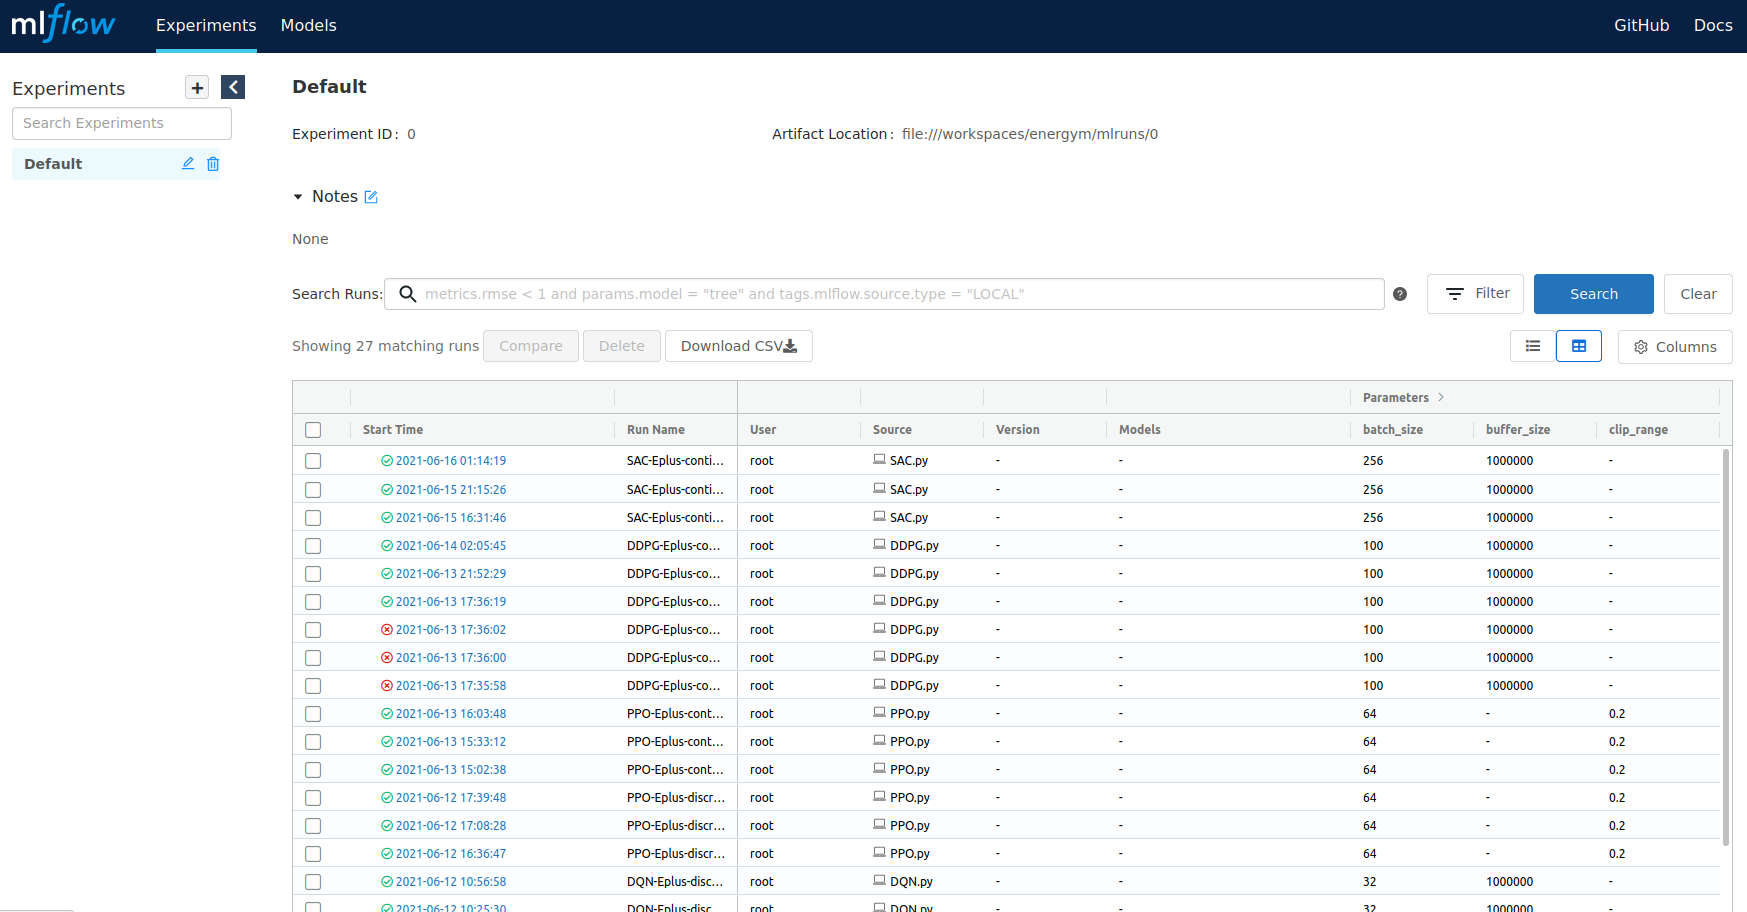
\includegraphics[width=\textwidth]{imagenes/mlflow.png}
    \caption{Experimentos registrados mediante MLflow}
    \label{fig:mlflow}
\end{figure}




